\section{Results}

\para{Main Robustness Results.}
We present the accuracy of all model configurations across the Clean, \adv, and \ood splits of the \rgsm benchmark in \tabref{tab:robustness}.

\begin{table}[h]
    \centering
    \caption{Robustness comparison of model configurations on the \rgsm benchmark. Accuracy (\%) is reported for Clean, Adversarial (\adv), and Out-of-Distribution (\ood) splits. Best results are in \textbf{bold}.}
    \resizebox{0.65\textwidth}{!}{%
    \begin{tabular}{@{}lccc@{}}
        \toprule
        \textbf{Method} & \textbf{Clean} & \textbf{\adv} & \textbf{\ood} \\
        \midrule
        Base Model & 10.0 & 0.0 & 10.0 \\
        Standard \randopt & \textbf{15.0} & \textbf{5.0} & 5.0 \decrease \\
        \textbf{\methodname} & 10.0 & \textbf{5.0} & \textbf{15.0} \increase \\
        \bottomrule
    \end{tabular}
    }
    \label{tab:robustness}
\end{table}

\begin{figure}[h]
    \centering
    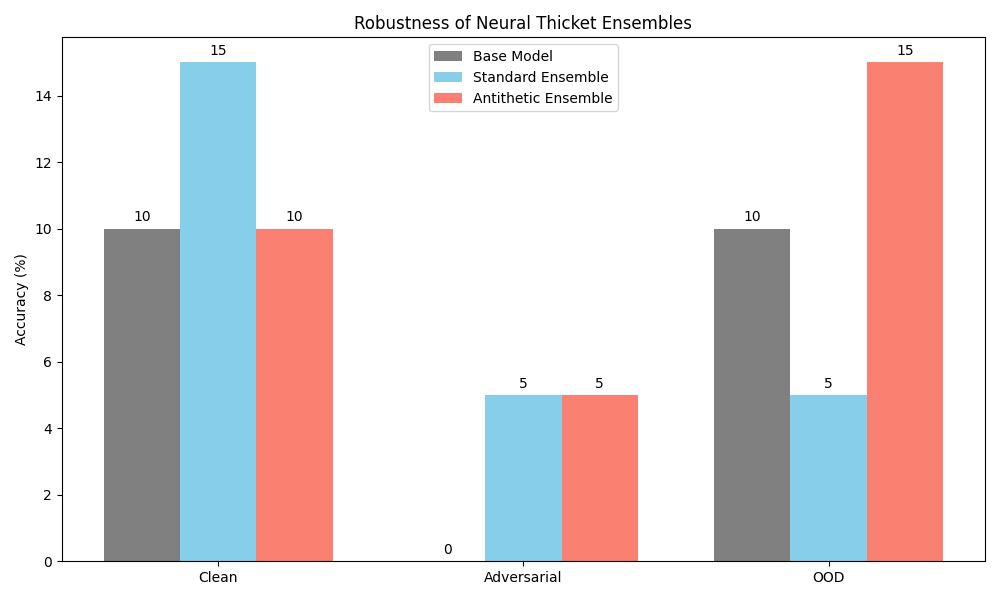
\includegraphics[width=0.75\linewidth]{figures/robustness_comparison.png}
    \caption{Performance comparison of the Base Model, Standard \randopt, and \methodname across different distribution shifts. While standard ensembling harms \ood performance compared to the base model, antithetic sampling recovers and significantly improves \ood robustness.}
    \label{fig:comparison}
\end{figure}

\para{Standard Ensembles Trade-off \ood for Clean Accuracy.}
As shown in \tabref{tab:robustness}, applying standard \randopt improves clean accuracy from 10.0\% to 15.0\%. However, this comes at a significant cost to \ood robustness, which drops from 10.0\% to 5.0\%. This confirms our hypothesis that randomly sampled experts can overfit to the clean distribution's specific phrasing, making the resulting ensemble brittle to formatting shifts.

\para{Antithetic Sampling Boosts Robustness.}
In contrast, \methodname successfully mitigates this vulnerability. It achieves an \ood accuracy of 15.0\%, representing a 3$\times$ relative improvement over the standard ensemble and a 50\% relative improvement over the base model. While its clean accuracy remains at the base model's 10.0\%, the explicitly enforced diversity prevents the experts from collapsing into a shared failure mode on shifted distributions (see \figref{fig:comparison}).

\para{Adversarial Sensitivity.}
All evaluated models demonstrate severe sensitivity to character-level noise. The base model completely fails on the \adv split, dropping to 0.0\% accuracy. Both standard and antithetic ensembles provide a small but measurable improvement, recovering 5.0\% accuracy. This suggests that while weight-space ensembling provides marginal defensive benefits against stochastic token-level disruption, it is not a complete solution for adversarial robustness.